\documentclass{beamer}
\beamertemplatenavigationsymbolsempty
\usecolortheme{beaver}
\setbeamertemplate{blocks}[rounded=true, shadow=true]
\setbeamertemplate{footline}[page number]
%
\usepackage[utf8]{inputenc}
\usepackage[english,russian]{babel}
\usepackage{amssymb,amsfonts,amsmath,mathtext}
\usepackage{subfig}
\usepackage{svg}
\usepackage[all]{xy} % xy package for diagrams
\usepackage{array}
\usepackage{multicol}% many columns in slide
\usepackage{hyperref}% urls
\usepackage{hhline}%tables

%----------------------------------------------------------------------------------------------------------
\title[\hbox to 56mm{Декодирование мозговых сигналов в аудиоданные}]{Декодирование мозговых сигналов в аудиоданные}
\author[Набиев М.\, Ф.]{Набиев Мухаммадшариф Фуркатович}
\institute{Московский физико-технический институт}
\date{\footnotesize
\par\smallskip\emph{Руководитель:} Северилов Павел Андреевич
% \par\smallskip\emph{Консультант:} Ш.\,Л.~Фоменко
\par\bigskip\small 2024}
%----------------------------------------------------------------------------------------------------------
\begin{document}
%----------------------------------------------------------------------------------------------------------
\begin{frame}
\thispagestyle{empty}
\maketitle
\end{frame}
%----------------------------------------------------------------------------------------------------
\begin{frame}{Декодирования мозговых сигналов в аудиоданные}
\footnotesize \textbf{Задача:} Классификация аудиостимулов на истинный и ложные. Истинным называется аудиостимул, который спровоцировал мозговую активность, сигнал которого мы получили.
\smallskip \smallskip 
\begin{columns}[c]
    \column{0.45\textwidth}
    \scriptsize \textbf{Формат данных:} Кортеж $(\mathbf{X}_i, \mathbf{s}_i^1, \dots, \mathbf{s}_i^k)$, где $\mathbf{X}_i \in \mathbb{R}^{64 \times m}$~--- ЭЭГ-сигнал, а $\mathbf{s}_i^1, \dots, \mathbf{s}_i^k \in \mathbb{R}^{1 \times m}$--- огибающие сигналов/стимулы.
    
    \column{0.55\textwidth}
    \scriptsize \textbf{Базовое решение:} Расширенная CNN ~--- энкодер, который переводит ЭЭГ и стимул в латентные пространства, где считается их близость.

\end{columns}
\smallskip \smallskip 
\scriptsize \textbf{Функция потерь:} Кросс-энтропия
$$CE = - \sum_{i=1}^N\sum_{k=1}^K y_i^k \log (\mathbf{F}(\mathbf{X}_i, \mathbf{s}_i^k)), \, \text {где $\mathbf{F}$~--- модель, а $y_i^k$~--- метка $k$-го стимула.}$$
\scriptsize Предлагается для ЭЭГ заменить CNN на трансформер и использовать физико-информированный энкодер для стимула, которые увеличат точность классификации.
% \bigskip
\begin{figure}
        \centering
        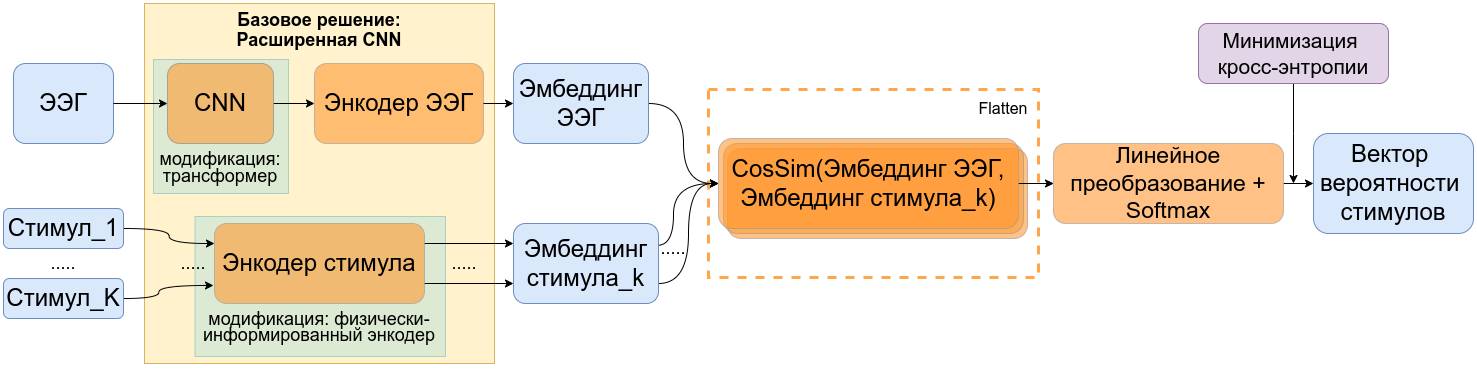
\includegraphics[width=0.90\textwidth]{model_architecture.png}
\end{figure}
% Важное {\color{red}сообщение}.
\end{frame}
%----------------------------------------------------------------------------------------------------
\end{document} 